\documentclass{article}
\usepackage{amsfonts}
\usepackage[T1,T2A]{fontenc}
\usepackage[utf8]{inputenc}
\usepackage[russian]{babel}
\usepackage{multicol}
\usepackage{graphicx}
\usepackage{natbib}
\usepackage{amsmath}
\usepackage{array}
\usepackage{mathrsfs}
\usepackage{pb-diagram}
\usepackage[noend]{algorithmic}
\usepackage{amssymb}
\usepackage{setspace}
\usepackage{appendix}
\usepackage{geometry}
\usepackage{color}
\usepackage[russian]{babel}
\bibliographystyle{unsrt}

\begin{document}
    
    \begin{figure}
        \centering
        
\includegraphics[scale=0.1]{logo.png}
    \end{figure}
    
    \begin{center}
        \begin{center}
            \line(1,0){300}
        \end{center}
    \hfill \break
    \large{Санкт-Петербургский государственный университет}\\ 
    \hfill \break
    \large{Математико-механический факультет}\\
     \hfill \break
   \normalsize{}{Прикладная математика и информатика}\\
    \hfill\break
    \hfill \break
    \large{Ковальчуков Александр Алексеевич}\\
    \hfill \break
    \hfill \break
    
    \hfill \break
    \hfill \break
    \hfill \break
    \large{Курсовая работа\\}
    \hfill \break
    \large{Обзор методов машинного обучения с учителем}\\
    \hfill \break
    \hfill \break
    \hfill \break
    \end{center}
     
     
     \begin{flushright}
        \normalsize{ 
            Научный руководитель \\
            к.ф.м.н,  доц.,  М.С. Ананьевский \\
            
        }
    \end{flushright}
    
    
    \vfill 
    \begin{center} Санкт-Петербург\\ 2019 \end{center}

\newpage


\section*{Введение}
    
    \begin{quote}
        \begin{flushright}
            Машинное обучение - облаcть исследований, которая наделяет компьютеры возможностью проявить поведение, которое не было заложено в них явно. \\
        \end{flushright}
    \end{quote} 
    
    \begin{flushright}
        Артур Сэмюэл, 1959 год$^\text{\citep{citation}}$
    \end{flushright}
    
    Эта работа написана с целью дать краткий обзор машинного обучения - одной из дисциплин искусственного интеллекта, возникшей в середине XX века на стыке информатики и статистики.
    Машинное обучение предоставляет медоды приближённого решения задач,  плохо или совсем не поддающиеся решению аналитическим путём. В основе этих методов лежат математические модели, которые обучаясь на наборах данных генерируют ассоциативные правила, позволяющие дать ответ на задачу в общем случае. Благодаря бурному развитию цифровой электроники, методы вышли за пределы лабораторий и получили широкое распространение в повседневной жизни. Так, персонализированная реклама, автокоррекция текста, машинный перевод и многие другие приложения в той или иной степени задействуют ML. Всплеск количества публикаций приходится на начало 2000, что можно соотнести с развитием интернета и накоплением разнообразных данных. 
    \hfill \break
    \hfill \break
    \hfill \break
    \hfill \break
    
    \begin{figure}[h]
        \center{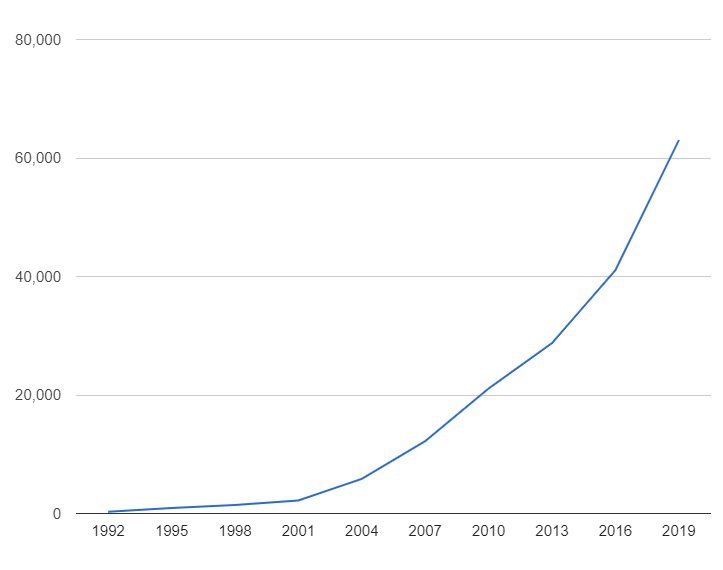
\includegraphics[scale=0.5]{stat.png}}
        
        \caption{ \centering График количества публикаций с 1992 по 2019 год. \\
        Построен по количеству побликаций в электронной библиотеке IEEE explore \\
        Запрос производился по ключевым словам ''machine learning''}
        \label{fig:stat}
    \end{figure}
    
    \newpage
    
\section*{Условные обозначения}
    \begin{itemize}
    \item \textbf{ML}: Machine Learning
    \item \textbf{AI}: Artificial Intelligence
    \item \textbf{ANN}: Artificial Neural Network
    \item \textbf{CNN}: Convolutional Neural Network
    \item \textbf{CPU}: Central Processor Unit
    \item \textbf{GPU}: Graphical Processor Unit
    
\end{itemize}

\section*{Мотивация}
    Как уже было сказано, основная область применения машинного обучения - это приближённое решение задач, и среди них принято выделять несколько основных:
    \begin{itemize}
        \item \textbf{Задача классификации} - отнесение объектов выборки к одному из нескольких классов по ассоциации с уже известными примерами.
        \item \textbf{Кластеризация} - выработка правила, упорядочевающего объекты исходной выборки в сравнительно однородные классы. Существенное различие с задачей классификации состоит в том, что модели не предоставляется тренировочных данных, а значит и никаких подсказок относительно искомой закономерности.
        \item \textbf{Задача регрессии} - поиск зависимости между значением целовой переменной и значениями одной или нескольких независимых величин.
        \item \textbf{Снижение размерности} - преобразование данных, состоящее в уменьшении числа признаков объекта путём получения главных переменных.
        \item \textbf{Ранжирование} - упорядочивание объектов по некоторому критерию. Нередко сводится к задачам классификации и регресии.
        \item \textbf{Фильтрация выбросов} - повышение качества исходной выборки для дальнейшего применения на чувствительных в выбросам моделей.
        
    \end{itemize}

\section*{Процесс машинного обучения}
    В общем контексте обучения с учителем процесс обучения можно описать как подбор функции  $f:X \rightarrow y$, которая адекватным образом соотносит входныеna данные $X$ значению целевой переменной $y$. \\
    \\
    Распространённый на практике процесс ML можно условно разделить на несколько стадий: 
    \begin{enumerate}
        \item Постановка задачи
        \item Добыча данных
        \item Подготовка данных 
        \item Подбор модели
        \item Обучение модели
        \item Проверка адекватности
        \item Анализ результатов
    \end{enumerate}
    Рассмотрим пункты 3 - 6 подробнее.
    \subsection*{Подготовка данных}
        Не все модели способны воспринимать данные в естественной форме, поэтому зачастую требуется серьезная предобработка данных и определение выбросов - качество модели напрямую зависит от полноты и чистоты тренировочной выборки. В задачи ML инженера входит очистка данных, их преобразование и нормализация.
        
    \subsection*{Подбор модели}
        Иногда выбор модели определяется поставленными задачами и форматом данных, однако порой оптимальных критериев подбора модели нет. В таких случаях приходится перебрать несколько моделей и выбрать из них лучшую, либо объеденить их в ансамбль.
        
    \subsection*{Обучение модели}
        На этом этапе происходит настройка внутренних параметров модели с целью приближения тренировочных данных. Все имеющие в распоряжении данные необходимо разбить на два непересекающихся набора: на одном модель будет обучаться в соответствии с её внутренними правилами, а на втором тестироваться. Особых рекомендаций по соотношению частей разбиения нет, хотя обычно модель обучают на 70\% данных, а тестируют на оставшихся 30\%. Но при этом чрезвычайно важно, чтобы данные в разбиении были представлены равномерно, чтобы обучение было объективным. В простейшем случае разбиение производится случайным образом.
        
    \subsection*{Проверка адекватности}
        На этом этапе модели на вход подаются данны, которые не были задействованы в процессе обучения, и по этим данным вычисляется общая ошибка модели.
        
        \subsubsection*{Матрица несоответствия}
            В случае классификации по всем тренировочной выборке составляется матрица $A$, $a_{ij}$ элемент которой показывает, сколько элементов класса $i$ были классифицированны как класс $j$. Сумма чисел на её главной диагонали показывает, сколько объектов было классифицированно правильно. По этой матрице можно извлечь численную оценку эффективности модели. Это может быть осуществлено разными способами.
            \begin{enumerate}
                \item \textbf{Точность и полнота} \\ 
                    В простейшем случае за такую величину можно принять отношение  правильно классифицированных объектов к размеру выборки: 
                    $$Accuracy = \frac{Tr(A)}{\sum a_{ij}}$$ 
                    Однако такая оценка оказывается необъективной, когда один класс в выборке встречается значительно чаще других, и модель хорошо работает только на нём получит хорошую оценку.
                \item \textbf{Точность и полнота} \\
                    Точность в пределах класса - это доля правильно классифицированных объектов среди всех ответов модели по данному классу:
                    $$Precision_k = \frac{a_{kk}}{\sum\limits_{i = 1}^n a_{i k}}$$
                    Полнота - это доля правильно классифицированных объектов данного класса среди объектов, действительно к нему относящихся.
                    $$Recall_k = \frac{a_{kk}}{\sum\limits_{j = 1}^n a_{kj}}$$
                    Точность и полнота всего классификатора вычисляется как среднее арифметическое точности и полноты ао всем классам.
                \item \textbf{$F_1$ - метрика} \\
                    В редких случаях удаётся одновременно достичь и точности и полноты одновременно. Если предпочтение отдаётся только точности или только, то проблемы нет - можно сравнивать модели по одному критерию. Но если важны оба критерия, то можно ввести метрику, равную среднему гармоническуму между точностью и полнотой:
                    $$F_1 = \frac{2}{\frac{1}{Precision} + \frac{1}{Recall}} = 2 \frac{Precision \times Recall}{Precision + Recall}$$
                    Такая величина стремится к 1, если точность и полнота одновременно стремятся к 1, и стремится к нулю, если хотя бы одна из этих величин стремится к нулю. 
            \end{enumerate}
        
        \subsubsection*{Среднеквадратическая ошибка}
            В случае регрессии индидикатором качества модели может служить среднеквадратическая ошибка. Чем она меньше, тем модель точнее.
            $$RMSE = \frac{\sum\limits_{i=1}^n(y_i - f(x_i))^2}{n}$$
        \subsubsection*{Cross-validation}
            Кросс-валидация - это техника валидации модели, позволяющая предсказать её работу на независимом наборе данных, при фактическом отсутствии такового. Один её цикл состоит в разбиении выборки на  2 части: на одной модель обучается, а на другой проверяется. Чтобы минимизировать ошибку, разные иттерации кросс-валидации производятся на разных разбиениях, а результаты валидации усредняются по всем циклам. Таким образом, модель можно обучать на всех имеющихся данных. \\
            Существует несколько распространённых типов кросс-валидации:
            \begin{enumerate}
                \item \textbf{По k блокам} \\
                    Исходный набор разбивается на k блоков, k-1 используются для тренировки, а 1 для валидации. Процесс повторяется k раз, причём блок валидации каждый раз меняется.
                \item \textbf{Поэлементная кросс валидация}
                    Представляется собой кросс-валидацию по k блокам, где k равно количеству объектов в выборке.
                \item \textbf{Валидация случайныйм сэмплированием}
                    На каждой иттерации выборка случайным образом разбивается на тренировочный и тестовый набор, но при этом некоторые объекты могут ни ни разу не попасть в тестовую выборку, а некоторые напротив - попасть в неё несколько раз.
            \end{enumerate}
            

\section*{Методы машинного обучения}
    Существует огромное количество моделей, заточенных под различные задачи, а   в пределах каждой из них существуют десятки различных вариаций. Я постараюсь дать обзор самых популярных из них.
    
    \subsection*{Линейная регрессия $^\text{\citep{Olap_and_Data_Mining}}$}
        Модель разработана задолго до наступления компьютерной эпохи, впервые появившись в работах Лежандра и Гаусса на рубеже XVIII и XIX веков.$^\text{\citep{Terms}}$ Суть состоит в определении линейной зависимости между одной целевой и несколькими независимыми переменными. Пусть анализируемый объект имеет n свойств: $x_1, x_2, \dots x_n$. Тогда значение целевой переменной определяется функцией
        $y = \omega_1 x_1 + \omega_2 x_2 + \dots + \omega_n x_n + \varepsilon$ с нормально распределённой случайной величиной $\varepsilon$. \\\\
        Пусть $y = \left(\begin{tabular}{c} $y_1$ \\ $y_2$ \\ $\vdots$ \\ $y_m$
        \end{tabular}\right)$ - вектор наблюдений зависимой переменной \\\\\\
        $X = \left(\begin{tabular}{c c c c} 
            $x_{11}$ & $x_{12}$ & $\dots$ & $x_{1n}$ \\
            $x_{21}$ & $x_{22}$ & $\dots$ & $x_{2n}$ \\
            \vdots & \vdots & \dots & \vdots \\
            $x_{m1}$ & $x_{m2}$ & $\dots$ & $x_{mn}$ \\
        \end{tabular}\right)$ - матрица признаков \\\\\\
        $\varepsilon = \left(\begin{tabular}{c} $\varepsilon_1$ \\ $\varepsilon_2$ \\ \vdots \\ $\varepsilon_m$
        \end{tabular}\right)$ - вектор случайных величин \\\\
        Тогда коэффициенты модели $\alpha$ являются решением неоднородной системы линейных уравнений \;\;\;
        $X \omega + \varepsilon  = y $
        
        
    \subsection*{Нелинейная регрессия}
        Реальные зависимости далеко не всегда хорошо описываются линейными моделями. В некоторых случаях может помочь нелинейная регрессия. \\
        Приведём некоторые часто используемые регрессионные модели:
        \begin{enumerate}
            \item Полиномиальная одномерная регрессия: $y = \sum\limits_{i = 0}^n \omega_i x^i$. Следует помнить, что полиномы высоких степеней склонны к переобучению
            \item Ряд Фурье: $y = a_0 + \sum\limits_{i = 1}^n (a_i \sin{(ix)} + b_i \cos{(bx)})$. Хорошо приближает периодические функции.
            \item Рациональный полином: $y = \frac{\sum\limits_{i = 0}^n a_i x^i}{\sum\limits_{j = 0}^m a_j x^j}$
            
        \end{enumerate}
        
    \subsection*{Наивный Байесовский классификатор \citep{rish2001empirical}}
        Модель получила своё название по теореме, лежащей в её основе. При классификации используется предположение о том, что все признаки в классе независимы. И хотя реальные признаки чаще всего коррелируют друг с другом, метод на удивление хорошо работает во многих ситуациях.
        Вероятностная модель устроена следующим образом: \\
        $P(y \;|\; X)$, где $X$ - вектор признаков. \\
        Используя теорему Байеса, формулу можно переписать в виде: \\
        $$P(y \;|\; X) = \frac{P(X \;|\; y)P(y)}{P(X)}$$
        И используя независимость признаков,
        $$P(y \;|\; X) = \frac{P(y)\prod\limits_{i=1}^n P(x_i \;|\; y)}{\prod\limits_{i = 1}^n P(x_i)}$$
        После выполнения модели объект относится к классу с наибольшей вероятностью. \\
        К достоинствам метода можно отнести высокую скорость обучения, небольшой размер обучающей выборки, а к недостаткам - достаточно грубое допущение о независимости переменных, а так же так явление, называемое нулевой частотой: если значение какого-то признака ни разу не встречалось в обучающей выборке, то такому явлению будет присвоена нулевая вероятность.
    
    \subsection*{Метод k-ближайших соседей \citep{elements_of_statistical_learning}}
        В основе метода лежит гипотеза компакности - предположение о том, что объекты одного класса похожи между собой: в пространстве объектов они образуют связную ограниченную область. Чтобы формализовать понятие похожести, на множестве объектов вводится метрика, адекватно оценивающая расстояние между объектами, причём её выбор целиком возлагается на плечи исследователя. \\
        Пусть $\rho(x_1, x_2)$ - метрика, $x$ - классифицируемый объект, а $x_{i_1}, x_{i_2}, \dots, x_{i_k}$ - $k$ ближайших к $x$ объектов. \\
        Тогда классифицируемый объект относится к тому классу, к которому относится большинство из его $k$ соседей. \\
        $$f(x) = arg \max\limits_{y \in Y} \sum\limits_{j = 1}^k [y(x_{i_j}) = y]$$.
        \\\\
        Модель также применима к задачам регресии. Восстановать значение целовой переменной в точке $x$ из пространства признаков можно взяв среднее арифметическое значений $k$ с оседних точек $x_{i_1}, x_{i_2}, \dots, x_{i_k}$:
        $$f(x) = \frac{1}{k} \sum\limits_{j = 1}^k y(x_{i_j})$$
        
        
    \subsection*{Метод опорных векторов \citep{Smola2004}} 
        SVM, или support vector machine, впервые примененялась для задач бинарной классификации. Рассмотрим объекты как точки в арифметическом векторном пространстве. В случае линейной разделимости классов можно провести гиперплоскость с наибольшим зазором, и все объекты но одну сторону гиперплоскости отнести к одному классу, а по другую - к другому. Максимизация зазора, то есть расстояние до ближайшего вектора, способствует более уверенной классификации \citep{vapnik2000bounds}. \\
        Пусть имеется выборка $(x_1, y_1), \dots, (x_k, y_k) x_i \in \mathbb{R}^n, y \in \{-1, 1\}$, и мы строим разделяющую гиперплоскость $w_1 x_1 + w_2 x_2 + \dots + w_n x_n + b = 0$, такую что для всех точек одного класса $\langle w, x_i \rangle + b > 0$, а для другого $\langle w, x_j \rangle + b < 0$. Объеденим два неравества в одно: $y_i(w, x_i \rangle + b) > 0$, и подберём константу $c$ таким образом, чтобы $с y_i(w, x_i \rangle + b) > 1$. \\
        % Поскольку при умножении на коПолучим $y_i(w, x_i \rangle + b) > 1 \;\; \forall i \in 1\dots k$
        //Доделать
        \\\\\\\\\\\\\
        Но случай линейной разделимости - большая редкость, и чаще всего выборку нельзя разделить линейно. Ключевой идеей, позволяющей применить SVM, будет перевод исходных векторов в пространство более высокой размерности, где они будут линейно разделимы.
        // доделать  
    \subsection*{Решающие деревья\citep{safavian1991survey}}
         Благодаря своей простоте и легкой интерпретируемости, решающее дерево является одной из самых распространённый моделей, используемых в машинном обучении. Оно представляет собой связный граф без циклов, в каждом промежуточном узле которого расположено решающее правило, а в листьях - метки классов. Деревья строятся так, чтобы по мере спуска классифицируемого объекта уменьшалась его классовая неопределённость.
         Для этого в корневой вершине происходит разбиение выборки $X$ на несколько частей $X_1, \dots X_k$, для каждой из которой вычисляется индекс неоднородности $H(X)$. Критерием качества разбиения служит уменьшение неоднородности: $\Delta H(X) = H(X) - \sum\limits_{i = 1}^k H(X_i) \frac{|X_i|}{|X|}$ - чем оно больше, тем лучше разбиение. 
         
         На практике часто используются следующие индексы неоднородности, где $K_1, K_2, \dots K_L$ - метки классов:
        \begin{itemize}
            \item Энтропийный индекс неоднородности: \\
                $H(X) = - \sum\limits_{i = 1}^L P(K_i) \log_2(P(K_i))$, \\
                где $P(K_i)$ - доля объектов класса $K_i$  в выборке $X$. При этом полагается, что $0\log_2 0 = 0$
            \item Индекс Джинни: \\
                $H(X) = 1  - \sum\limits_{i = 1}^L P(K_i)^2$
            \item Индекс ошибочной классификации: \\
                $H(X) = 1  - \max\limits_{1 \dots L} P(K_i)$
        \end{itemize}
        Как видно, минимум индекcа неоднородности достигется при принадлежности всех объектов выборки к одному классу. \\
        Далее алгоритм рекурсивно применяется к потомкам вершины, только в качестве выборки служит один из полученных элементов разбиения. Построение дерева прекращается когда будет достигнут один из критериев останова:
        \begin{itemize}
            \item Все объекты в вершине имеют один класс
            \item Достижение максимальной глубины дерева
            \item Достижение ограничения на минимальное количество объектов в вершине 
            \item Достижение максимального числа листьев
            \item Слишком малое уменьшение неопределённости.
        \end{itemize}
        При использовании первого критерия останова будет построено дерево, которое абсолютно точно классифицирует объекты тренировочной выборки, однако оно может оказаться очень глубоким и совершенно не отражать реальных зависимостей, в результате чего на тестовой выборке оно покажет плохой результат. Такая систуация называется переобучением (overfitting). Избежать переобучения позволяет подрезка деревьев. \\
        Применим построенное дерево к тренировочной выборке и рассмотрим вершину $t$. Если до $t$ не дошёл ни один объект тестовой выборки, то такая вершина неинформативная, и её можно заменить на лист с меткой, соответствующей самому частому классу в поддереве по тренировочной выборке. Если же до $t$ дошли объекты тестовой выборки, то надо вычислить число ошибок на ней и на каждом из её поддеревьев. Если какое-либо из поддеревьев совершает меньше ошибок, то следует заменить $t$ на это поддерево, а остальные отсечь.
        \\\\
        Решающие деревья также можно применять для регрессии, только вместо меток классов в лисьях будут храниться значения целевой переменной.
        
    \subsection*{Ансамблирование}  
        Пусть у нас есть семейство \textit{слабых класссификаторов}$^\text{\citep{lienhart2003empirical}}$(тех, у которых вероятность правильного ответа немного превышает случайную). Тогда если усреднить их ответы на произвольном объекте, то точность увеличится по сравнению с одиночным классификатором. А именно, если вероятность правильного ответа одного дерева $P_i > 0.5$, то вероятность ошибки ансамбля равна $\prod\limits_{i = 1}^n (1 - P_i)$ и она уменьшается по мере роста числа деревьев. Построение таких ансамблей оказалось чрезвычайно эффективным и значительно превосходящим многие другие методы ML.
        
        \subsubsection*{Бэггинг \citep{breiman1996bagging}}
            Одна из ранних версий ансамблей, придуманная Лео Брейманом в 1994 году. В основе бэггинга лежит процедура бутстрепа - выборки с повторениями. Из множества исходных данных отбирается несколько подвыборок, размер которых совпадает с размером исходного множества. Так как отбор происходит случайным образом, то некоторые объекты могут попасть в одну и ту же выборку несколько раз, а в некоторые не попасть вовсе. \\ \\
            \textit{Если размер выборки равен $n$, каждый объект имеет шанс $\frac{1}{n}$ попасть в неё. Вероятность того, что он не попадёт в выборку равна $(1 - \frac{1}{n})^n \rightarrow \frac{1}{e} \approx 0.36$ при $n \rightarrow \infty$}  \\
            Таким образом каждая подвыборка имеет в среднем $\frac{2}{3}$ уникальных объектов.
            \\\\
            Затем на выборках $X_1, X_2, \dots, X_l$ полученных в результате бутстрепа обучается отдельный классификатор, который затем будет участвовать в голосовании для определения класса. \\
            Следует отметить, что на больших данных, характерных для машинного обучения, метод не гарантирует отсутствия корреляции между деревьями. Поэтому он получил дальнейнее развитие в более поздних статьях Лео Бреймана.
                
        \subsubsection*{Случайный лес \citep{Random_Forests}} 
            Модель является усовершенстованием бэггинга. Она также состоит из бутстрепа и построении деревьев по подвыборкам с повторениями, только в этот раз для каждого дерева установлено ограничиние в k признаков, которые могут использоваться для обучения, из n исходных. Затем голосованием деревьев объект относится к самому популярному классу. Случайный лес, как и бэггинг хорошо распараллеливаются, позволяя быстро получать модели с хорошей точностью.
        
        \subsubsection*{Out-of-bag оценка} 
            Поскольку тренировочные данные используются неравномерно, при поверке адекватности ансамбля нет необходимости использовать отдельный набор тестовых данных или кросс-валидацию. Можно оценить ошибку отдельного дерева по $36\%$ данных, которые в неё не попали. Это даёт нам оценку на весь ансамбль.
        
        \subsubsection*{AdaBoost \citep{freund1997decision}}
            Алгоритм построения сильного классификатора, предложенный Йоавом Фройндом и Робертом Шапиром в 1996 году. Алгоритм последовательно стоит взвешенный ансамль из деревьев глубины 1 (т.н. "пней"), придавая особое значение тем объектам, которые плохо распознаются предыдущими версиями ансамбля.
            Рассмотрим пример работы алгоритма в задаче бинарной классификации:
            Пусть $(x_1, y_1), \dots, (x_k, y_k)$ - тренировочная выборка, где метка класса приминает 2 значения: $y \in \{-1, 1\}$. \\
            Первоначально все объекты выборки имеют одинаковый вес: \\
            $w_0(x_i) = \frac{1}{m}$ \\
            Алгоритм состоит из $T$ иттераций. На $t$ иттерации: \\
            \begin{itemize}
                \item Строится пень $h_t(x)$, минимизирующий взвешенную ошибку выборки $\varepsilon$.
                \item Вычисляется $\alpha_t = \frac{1}{2}\ln \frac{1 - \varepsilon}{\varepsilon}$ - значимость $t$ классификатора. При $\varepsilon \rightarrow 0.5$  $\alpha_t \rightarrow 0$ 
                \item Веса объектов обновляются и нормализуются, чтобы получить распределение вероятностей. 
                $w_{t+1}'(i) = w_t(i)e^{- \alpha_t y_i h_t(x_1)}$ \\
                $s = \sum\limits_{i = 1}^n w_{t+1}' (i), \;\; w_{t+1} (i) = \frac{w_{t+1}' (i)}{s}$ \\
                При этом вес правильно классифицированных объектов уменьшается по отношению к весу неправильно классифицированных.
            \end{itemize}
            В результате выполнения алгоритма получается взвешенный ансамбль
            $f(x) = sign \left( \sum\limits_{i = 1}^T \alpha_t h_t(x) \right)$
            \\\\
            AdaBoost также применим к задачам множественной классификации, регрессии и ранжирования, однако в отличии от Бэггинга и Случайного леса, не распараллеливается. 
            
    \subsection*{Градиентный бустинг}
        Как и AdaBoost, градиентный бустинг строит сильную модель последовательным добавлением более слабых моделей, обычно деревьев решений.
        
        Модель будем строить в виде $f(x) = \sum\limits_{t = 1}^T h_t(x)$, где $h_t(x)$ - дерево решений небольшой глубины.
        Для оценки качества алгоритма необходимо минимизировать функцию потерь: $L(y, z)$, где $y$ - правильных ответов, $z$ - прогнозы классификатора. Для регрессии подойдёт среднеквадратическая ошибка: $L(y, x) = \frac{1}{л} \sum$
    
    \subsection*{Нейронные сети}
        \subsubsection*{Перцептрон \citep{rosenblatt1958perceptron}}
            
    
    \subsection*{Глубокое обучение \citep{Deep_learning}}
    
    \subsection*{Генетические алгоритмы \citep{deb2002fast}}
        Генетические алгоритмы используются в задачах оптимизации и моделирования и заимствуют идеи из эволюционного процесса живых организмов - в их осневе лежат мутации, скрещивание и естественный отбор. \\\\
        Решением задачи оптимизации является особь с наилучшим значением функции приспособленности (fitness), параметрами которой являются её гены, обычно представляемые в виде вектора фиксированной длины.  \\\\
        В качестве первого приближения случайным образом генерируется популяция размера $n$ (не обязательно конкурентоспособная, но достаточно генетически разнообразная), затем начинается иттеративный эволюционный процесс. \\\\
        На каждом шаге алгоритма поочерёдно применяются следующие операторы:
        
        \subsubsection*{Оператор селекции}
            Аналог естественного отбора в природе. В простейшем случае из полуляции выбирают $k$ наиболее приспособленных особей, чье потомство войдёт в следующее поколение. Однако такой подход может привести к ситуации, когда через несколько поколений весь генотип будет происходить от одного предка и вся популяция застрянет около локального оптимума. Избежать проблемы генетического однообразия позволяет алгоритм NSGA-II: \\
            Пул особей для размножения формируется не из наиболее приспособленых, из наиболее редких, то есть из тех, евклидово расстояние между которыми велико. Затем к отобранным особям применяется оператор скрещивания, и из полученных $2n$ особей выбираются наиболее приспособленные. 
            
        \subsubsection*{Оператор скрещивания}
            Обычно скрещивание происходит над двумя особями $x = (x_1, x_2, \dots, x_l)$ и $y = (y_1, y_2, \dots, y_l)$ и образует двух потомков. В зависимости от реализации, оно может быть
            \begin{itemize}
                \item одноточечным \\ 
                    (потомки будут иметь вид $a = (x_1, \dots x_k, y_{k+1}, \dots, y_l)$ и $b = (y_1, \dots y_k, x_{k+1}, \dots, x_l)$ \\
                    точка $k \in 1 \dots l$ выбирается случайно)
                \item двухточечным \\
                    $a = (x_1, \dots x_k, y_{k+1}, \dots, y_m, x_{m+1}, \dots x_l)$ и $b = (y_1, \dots, y_k, x_{k+1}, \dots, x_m, y_{m+1}, \dots, y_l)$
                \item по произвольной битовой маске, где $i$ ген отнесётся к первому потомку, если $i$ бит маски 1, и ко второму в противном случае.
            \end{itemize}
            В некоторых реализациях возможно скрещивание с использованием трёх и более родителей.
        \subsubsection*{Оператор мутации}
            Применимо к конкретной особи, оператор меняет один или несколько генов на некоторую величину. Позволяет добиться большего генетического разнообразия или выйти из локального экстремума.
        \\\\\\\
        Эволюция останавливается, когда будет достигнут один из критерий останова:
        \begin{itemize}
            \item Нахождение глобального или локального решения
            \item Достижение максимального числа поколений
            \item Превышение времени работы алгоритма
        \end{itemize}

\section*{Результаты, достигнутые в области}
    Большинство из используемых на сегодняшний день методов машинного обучения были разработаты ещё в 60-е годы XX века, но повсеместное их использование началось во втором десятилетии XXI века, когда человечество накопило большое количество информации, а вычислительные мощности стали дешёвыми.
    
    Наиболее существенными существенные достижения в области за последние 10 лет: 
    
    \subsection*{Распознавание речи}
            Согласно исследованию Microsoft\citep{xiong2016achieving}, проведённому на датасете NIST 2000, в 2016 году системы распознавания речи достигли человеческого уровня. В разговорах малознакомых людей на заданную тему точность распознавания составила $5.8\%$, а в неформальных разговорах друзей и родственников - $11\%$, что на $0.1\%$ и $0.3\%$ больше точности профессиональных стенографистов. Добиться такой точности помогла комбинация CNN и RNN с долгой краткосрочной памятью.
            
    \subsection*{Синтез речи}
    
    \subsection*{Распознавание образов}
    
    \subsection*{Медицинская диагностика}
        Потенициал применения AI в медицине довольно велик, о чём свидетельствует ???, однако его использование сопряжено с рядом трудностей:
        \begin{itemize}
            \item Плохая интерпретируемость некоторых моделей
            \item Трудность сертификации
            \item Отсутствие доверия у населения
        \end{itemize}
        В связи с чем большинство решений позиционирует себя не как полную замену врачу, а как систему поддержки принятия решений.
        К числу наиболее заметных работ последних лет можно отнести работы Стенфордского университета \citep{rajpurkar2017chexnet} по классификации рентгенограмм пациентов. Модель на основе CNN способна диагностировать одно из 14 заболеваний, а пневмонию она определяет лучше врачей-рентгенологов.
        
    \subsection*{Кредитный скоринг}
        Нет достоверной информации. 
    \subsection*{Распознование рукописного ввода}
    
    \subsection*{Обнаружение спама}
        В задачах фильтрации спама хорошо зарекомендовал себя Байесовский классификатор \citep{androutsopoulos2000evaluation}. При обучении классификатора высчитывается вероятность, что письмо с данным словом - спам, а при классификации нового письма, вероятность того, что оно является спамом оценивается через вероятности составляющих его слов. Метод не требует больших вычислительных ресурсов, способен дообучаться и показывает 95-97\% точность, за счет чего лежит в основе большинства современных спам-фильтров. 
    \subsection*{Улучшение качества изображений}
    
    
    \subsection*{Улучшение качества видео}
        Рост производительности персональных компьютеров и в частности, GPU, позволил \citep{shi2016real} в реальном времени применять интерполяционные алгоритмы на основе CNN для повышения качества видео с минимальными потерями детализации. 
        
    \subsection*{Голосовые ассистенты \citep{10.1007/978-3-319-60366-7_23}}
        Современные голосовые ассистенты, встроенные в операционную систему или программное обеспечение наиболее близко подобрались с понятию искусственного интеллекта. Они решают срезу несколько задач: speech-to-text преобразование, семантический анализ текста, запросы к сервисам, преобразование ответа обратно в речь. По заявляниям Яндекса \citep{yandex2018conf}, спрос на голосовых помощников постоянно растёт, и по состоянию на май 2018 года, голосовой асссистент <<Алиса>> установлена на 53\% российских сматрфонах и доступна в навигаторах 20 млн автомобилей.

\bibliographystyle{plain}
\bibliography{references}


\end{document}